% !TEX root = ../../I4PRJ, Grp3 - Rapport.tex
\chapter{Specifikation og Analyse}\label{SpecOgAnalyse}
Afsnittet beskriver specifikations- og analysearbejdet. Specifikationsarbejdet begyndte med analyse af projektformulering. Analysen bestod af at løse de problemstillinger, som projektformuleringen rejser ved hjælp af user stories. User stories, ses i det tidligere afsnit~\ref{FunkKrav}. User stories blev prioriteret ved en MoSCoW analyse, som også fremgår i tabel~\ref{table:functional}. Til at danne overblik over systemets domæner, foretog gruppen en domæneanalyse af user stories. Resultatet af analysen ses på figur~\ref{fig:domainmodelboundary}.

\begin{figure}
	\centering
	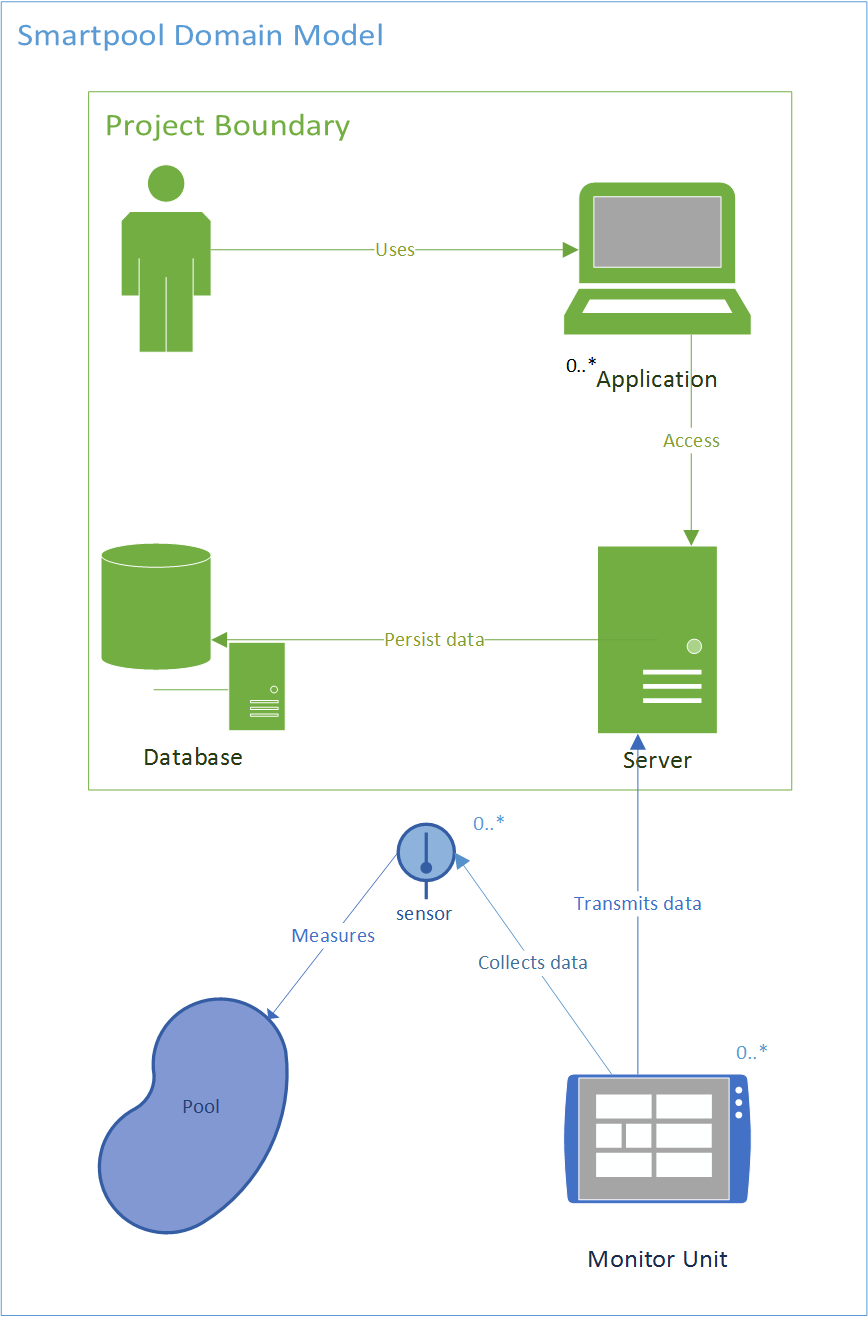
\includegraphics[width=0.6\linewidth]{figs/ProjectBoundary}
	\caption{Domænemodel for systemet}
	\label{fig:domainmodelboundary}
\end{figure}

Smartpool projektet afgrænses til at være foruden dataopsamlingsdelen, hvilket også er vist i Figur~\ref{fig:domainmodelboundary}. Dette vises med en grøn markering af de dele projektet kommer til at indeholde.

For en domænebeskrivelse se dokumentationen afsnit Domænebeskrivelser under Kravspecifikation.

Specifikations- og analysearbejde er ligesom alt andet i projektet en iterativ proces. Det betyder, at de user stories som er defineret i denne rapport, ikke nødvendigvis er de samme, som da udviklingsprocessen startede. Undervejs i denne proces har såvel domæneanalysen og -modellen ændret sig.

Et eksempel på udfærdigelse af et kvalitetskrav er, udarbejdelse af et ensartet visuelt design. Alle GUI's skal fremstå ens uanset platform. Det betyder både i funktionalitet, men også i fremtoning. Kvalitetskravet blev opfyldt ved at lave et konceptuelt design (se figur~\ref{fig:conceptualdesignview}), som blev udviklet til et grafisk design (se figur~\ref{fig:graphicaldesign}). For at sikre ensartethed udarbejdedes en farvepalet (se tabel~\ref{table:farvepalet}).

% !TEX root = ../../../I4PRJ, Grp3 - Rapport.tex
\chapter{Grafisk Design}
I dette afsnit beskrives det grafiske design af brugergrænsefladen. Det grafiske design skal afspejle de respektive views funktionalitet. Først udarbejdes et konceptuelt design. GUI views designes ved at analyserer og diskuterer user stories for systemet. Resultatet af analysen er et håndtegnet design med tilhørende noter fra diskussionerne. Analyseresultatet dannede grundstenene for GUI folkenes arbejde. Designet blev dermed ensartet for de forskellige platforme. Det fælles udarbejdede design har mindsket en muligt senere kommende bureaukratisk proces, da alle udviklere ved at målet er nået, når GUI svarer til design. 

\section{Konceptuel Design}
Først udarbejdes et konceptuelt design. Det konceptuelle design udarbejdes ved analyse og diskussion af user stories, som eksempel er user story omhandlende login behandlet og kan ses på figuren nedenfor:

\begin{figure}
	\centering
	\includegraphics[width=\linewidth]{figs/design/konceptuel_design_loginview}
	\caption{Domænemodel for systemet}
	\label{fig:domainmodel}
\end{figure}

De forskellige platformes GUI minder i så høj grad om hinanden, at hvert view og hvilke user stories de implementerer kun vil blive beskrevet for en platform. 
\subsection{Farvepalet}
For at opfylde kvalitetskravet, at applikationer skal være visuelt ensartede, er der under det visuelle design lavet en Smartpool farvepalet.
\begin{table}[]
\centering
\begin{tabular}{ll}
SpBlack          & \cellcolor[HTML]{0A0A0A}{\color[HTML]{FFFFFF} \#FF0A0A0A} \\
SpDarkGrey       & \cellcolor[HTML]{1F1F1F}{\color[HTML]{FFFFFF} \#FF1F1F1F} \\
SpGrey           & \cellcolor[HTML]{575757}{\color[HTML]{FFFFFF} \#FF575757} \\
SpLightGrey      & \cellcolor[HTML]{ABABAC}\#FFABABAC                        \\
SpOrange         & \cellcolor[HTML]{FDA029}\#FFFDA029                        \\
SpRed            & \cellcolor[HTML]{FF584D}\#FFFF584D                        \\
SpLightBlue      & \cellcolor[HTML]{49BAE1}\#FF49BAE1                        \\
SpBlue           & \cellcolor[HTML]{0354A5}\#FF0354A5                        \\
SpWhite          & \cellcolor[HTML]{FFFFFF}\#FFFFFFFF                        \\
SpBackgroundGray & \cellcolor[HTML]{2E2E2E}{\color[HTML]{FFFFFF} \#FF2e2e2e} \\
SpAccentGray     & \cellcolor[HTML]{3E3E3E}{\color[HTML]{FFFFFF} \#FF3e3e3e}
\end{tabular}
\caption{Farvepalet}
\label{table:farvepalet}
\end{table}

